% Created 2021-01-25 Mon 09:59
% Intended LaTeX compiler: pdflatex
\documentclass[presentation]{beamer}
\usepackage[utf8]{inputenc}
\usepackage[T1]{fontenc}
\usepackage{graphicx}
\usepackage{grffile}
\usepackage{longtable}
\usepackage{wrapfig}
\usepackage{rotating}
\usepackage[normalem]{ulem}
\usepackage{amsmath}
\usepackage{textcomp}
\usepackage{amssymb}
\usepackage{capt-of}
\usepackage{hyperref}
\usetheme{UoB}
\author{Mark Blyth}
\date{\textit{[2021-01-25 Mon]}}
\title{More BSpline struggles}
\hypersetup{
 pdfauthor={Mark Blyth},
 pdftitle={More BSpline struggles},
 pdfkeywords={},
 pdfsubject={},
 pdfcreator={Emacs 27.1 (Org mode 9.3)}, 
 pdflang={English}}
\begin{document}

\maketitle

\section{Background}
\label{sec:org049e47e}
\begin{frame}[label={sec:org4d937ae}]{Week's work}
Last time:
\begin{itemize}
\item Adaptive stepsizes might fix everything
\end{itemize}
\vfill
This time:
\begin{itemize}
\item Adaptive stepsizes are lots of hassle for little benefit
\begin{itemize}
\item BUt that's an interesting insight in itself!
\end{itemize}
\item Jacobian computation has a large impact on results
\end{itemize}
\end{frame}

\section{Stepsizes}
\label{sec:orge478bc4}
\begin{frame}[label={sec:org1563e84}]{Some convergence issues}
\begin{itemize}
\item Before adaptive stepsizes, I used a single Newton iteration for speed
\begin{itemize}
\item Adaptive stepsizes requires 2+ Newton iterations; ran until convergence, instead of taking a single step
\end{itemize}
\end{itemize}
\vfill
\begin{itemize}
\item With more Newton steps, the iterations diverge at the fold
\begin{itemize}
\item Taking more steps leads to exponentially more wrong solutions
\item Also implemented Newton-Broyden; same thing happens
\end{itemize}
\end{itemize}
\vfill
\begin{itemize}
\item The same thing happens with and without adaptive stepsizes
\begin{itemize}
\item Taking a single Newton step works
\item Taking more steps causes exponentially fast divergence at the fold
\end{itemize}
\end{itemize}
\vfill
\begin{itemize}
\item Stepsizes adapt a lot, suggesting convergence properties change rapidly along the curve
\end{itemize}
\end{frame}

\begin{frame}[label={sec:orgcc6cfba}]{Hypothesis 1}
BSplines are a bad way of representing the signal
\begin{itemize}
\item Fourier is a natural description of the signal; fundamental harmonic describes amplitude, the rest describe shape
\item Maybe splines don't caputure the signal well, and
\item If so\ldots{}
\begin{itemize}
\item Small changes in the signal give big changes to BSpline discretisation
\item Continuation curve is very wiggly in discretisation-space?
\item Tangent prediction becomes a fairly useless starting point
\end{itemize}
\end{itemize}
\vfill
Test: look successive BSpline coefficients
\vfill
Result: they change nice and smoothly; probably not an issue; hypothesis rejected
\end{frame}

\begin{frame}[label={sec:org1cc8e46}]{Hypothesis 2}
The system has not converged to a stabilised PO at divergence points

\begin{itemize}
\item Doesn't make sense to discretise transients
\item If the system hasn't converged, the IO-map evaluation, and therefore predictor-corrector calculations, are meaningless
\end{itemize}
\vfill
Test: plot the control target and system output after tangent prediction
\vfill
Result: at tangent-prediction, the PO has always converged; probably not an issue; hypothesis rejected
\end{frame}
\begin{frame}[label={sec:orge11f5b3}]{Other problem}
Struggles to converge on second SPO branch; jumps randomly, happens to be in the right direction

\begin{center}
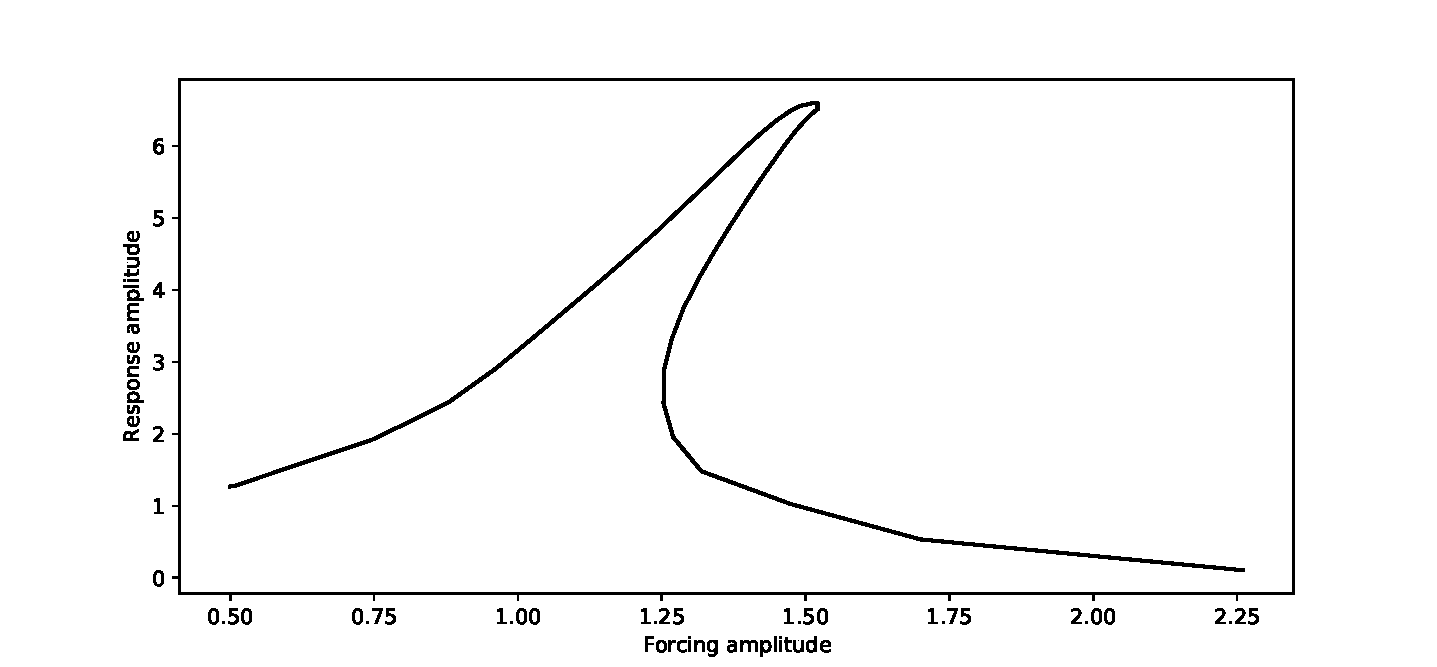
\includegraphics[width=.9\linewidth]{./nonadaptive_onestep-newton_dsize5_fdss_none_stepsize1.pdf}
\end{center}
\end{frame}


\begin{frame}[label={sec:org03425a6}]{Faster Jacobian method}
\begin{center}
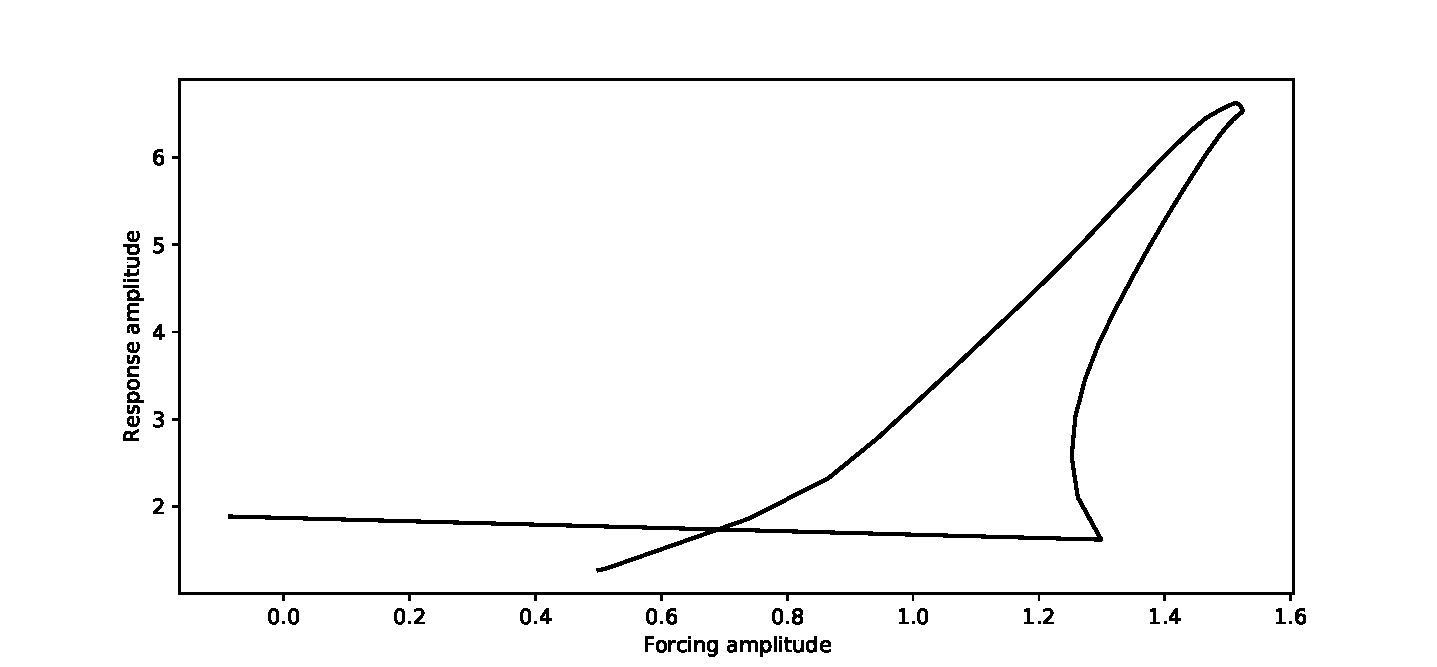
\includegraphics[width=.9\linewidth]{./kp1_transtime100_newton.pdf}
\end{center}

Identical setup but slightly different Jacobian computation
\end{frame}

\begin{frame}[label={sec:orgb48b033}]{Even faster Jacobian method}
\begin{center}
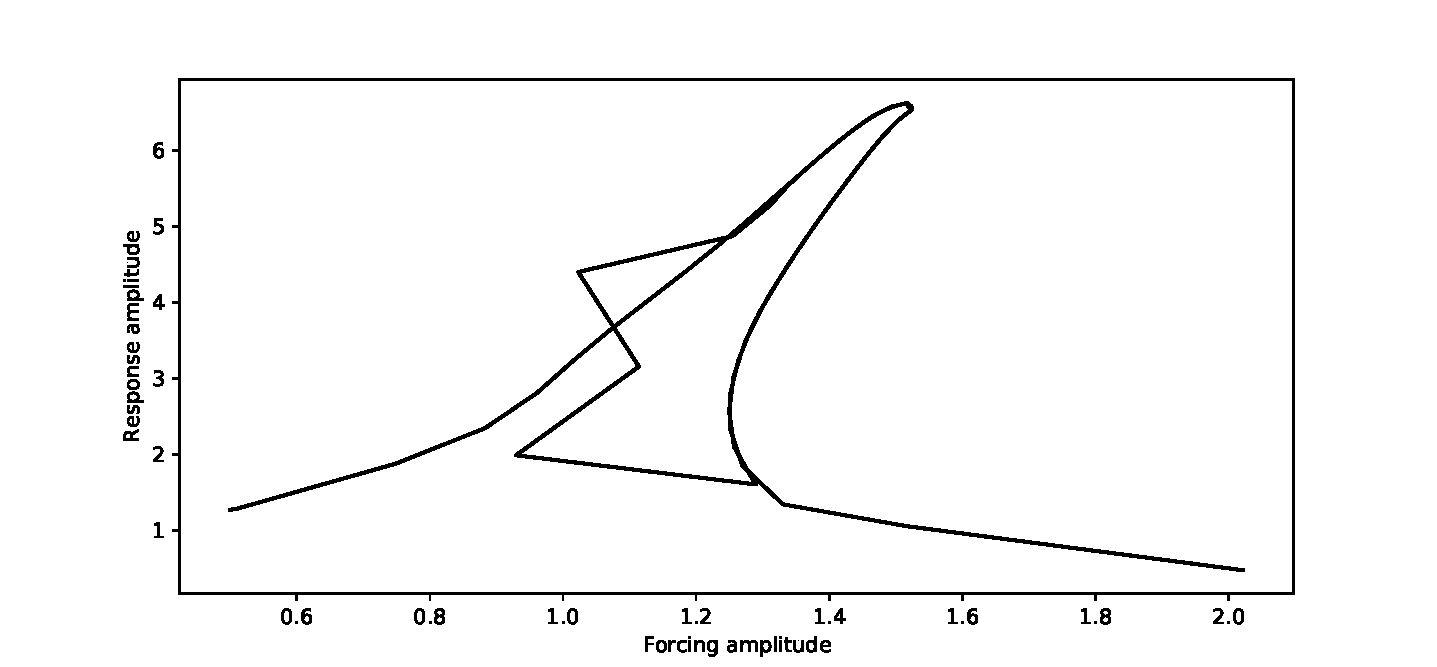
\includegraphics[width=.9\linewidth]{./nonadaptive_onestep-newton_dsize5_my_jacobian_fdss_0d2_stepsize1.pdf}
\end{center}

Another identical setup, new Jacobian. Looks like solution repels the Newton interations; doesn't entirely make sense
\end{frame}

\begin{frame}[label={sec:org89212d0}]{Hypotheses 3, 4}
Solution fails to converge, and jumps randomly
\begin{itemize}
\item Sometimes we get lucky and it jumps back to the curve
\item Not really working properly!
\end{itemize}
\vfill
Either
\begin{itemize}
\item Jacobian is somehow problematic
\begin{itemize}
\item First Newton step succeeds, so initially the Jacobian is probably right
\end{itemize}
\end{itemize}
or
\begin{itemize}
\item Continuation equations are misbehaving
\begin{itemize}
\item Broyden only uses the initial Jacobian, and updates from function values
\item Broyden shows same divergence; presumably it's the function values at fault
\end{itemize}
\end{itemize}
\vfill
\end{frame}


\begin{frame}[label={sec:org3b331bb}]{Computational setup}
All approaches use single Newton iterations; difference here is in the Jacobian computation; three methods tested:
\vfill
\begin{itemize}
\item Pre-made numdifftools
\begin{itemize}
\item Adaptive FDSS; should give best results
\item Slow; 1h 8 minute runtime
\end{itemize}
\item Pre-made numdifftools
\begin{itemize}
\item Fixed FDSS; more potential for inaccuracy
\item Faster run-time
\end{itemize}
\item Simple DIY finite differences with fixed FDSS
\begin{itemize}
\item Forward or central-step finite differences
\item 7 minute run-time
\end{itemize}
\end{itemize}
\end{frame}

\begin{frame}[label={sec:org01679d2}]{Jacobian computation}
Forward:
\[J[i,j] = \frac{f_i(x + h e_j) - f_i(x)}{h}\]
Central:
\[J[i,j] = \frac{f_i(x + h e_j) - f_i(x - h e_j)}{2h}\]
\vfill
Forward: \(n+1\), central: \(2n\) function evaluations, for \(x\in\mathbb{R}^n\)
\end{frame}

\begin{frame}[label={sec:org82418a8}]{Jacobian accuracy}
Changing FDSS has a big effect on the Jacobian
\begin{itemize}
\item Needs to be very large to get results reliably
\item Typically would use \(\mathcal{O}(10^{-6})\) steps; I use 0.2
\item Changing stepsize has a large impact on Jacobian
\end{itemize}
\vfill
Changing between central and forward has a big effect on Jacobian
\begin{itemize}
\item Changing between forward and central changes some entries by 10\%
\end{itemize}
\vfill
Can't reliably take correct Newton steps if we can't find an accurate Jacobian
\end{frame}

\begin{frame}[label={sec:org92e344d}]{Some issues}
\begin{itemize}
\item No idea why this happens with splines but not Fourier
\end{itemize}
\vfill
\begin{itemize}
\item Can't spot an easy way to test if the Jacobian is the problem
\begin{itemize}
\item Broyden results suggest its more likely down to the continuation equations
\item Misbehaving continuation equations would also make it harder to compute a Jacobian
\end{itemize}
\end{itemize}
\vfill
\begin{itemize}
\item If Jacobian isn't the problem, the continuation equations are misbehaving
\begin{itemize}
\item Eg. solution has a very small basin of attraction
\item This is easier to test: try collocation -- different continuation equations
\end{itemize}
\end{itemize}
\vfill
\begin{itemize}
\item Different continuation equations might help both the solution behaved-ness and Jacobian computation
\end{itemize}
\end{frame}

\section{Next steps}
\label{sec:org660aaef}
\begin{frame}[label={sec:orgc7eace8}]{Next steps}
This week:
\vfill
\begin{itemize}
\item Reading, writing, NODYCON presentation
\end{itemize}
\vfill
Then\ldots{}
\begin{itemize}
\item Ignore the problem!
\begin{itemize}
\item Tried lots of ideas and it's still not working properly
\item I'm not convinced I can gain any further insights with the current simulate-and-test method
\end{itemize}
\item Implement a phase condition, and test BSpline CBC with a different system
\item If that doesn't work either, try BSpline collocation
\begin{itemize}
\item All the usual BSpline benefits
\item Hopefully more numerical stability
\item Less noise robustness (but that can be overcome!)
\end{itemize}
\end{itemize}
\end{frame}
\end{document}
